%%%%%%%%%%%%%%%%%%%%%%%%%%%%%%%%%%%%%%%%%%%%%%%%%%%%%%%%%%%%%%%%%%
%%%%%%%% ICML 2017 EXAMPLE LATEX SUBMISSION FILE %%%%%%%%%%%%%%%%%
%%%%%%%%%%%%%%%%%%%%%%%%%%%%%%%%%%%%%%%%%%%%%%%%%%%%%%%%%%%%%%%%%%

\documentclass{article}
\usepackage{times,graphicx,subfigure,natbib,algorithm,algorithmic,hyperref}
\usepackage{amsmath,amsthm,amssymb,enumitem,verbatim}
% Packages hyperref and algorithmic misbehave sometimes.  We can fix
% this with the following command.
\newcommand{\theHalgorithm}{\arabic{algorithm}}
\newcommand{\simiid}{\overset{\textrm{i.i.d.}}{\sim}}
\newcommand{\mE}{\mathbb{E}}
\DeclareMathOperator*{\argmin}{arg\,min}
\newtheorem{lemma}{Lemma}
\newtheorem{theorem}{Theorem}
\newtheorem{corollary}{Corollary}
\graphicspath{{figures/}{../figures/}}

% Employ the following version of the ``usepackage'' statement for
% submitting the draft version of the paper for review.  This will set
% the note in the first column to ``Under review.  Do not distribute.''
\usepackage{icml2017} 

% Employ this version of the ``usepackage'' statement after the paper has
% been accepted, when creating the final version.  This will set the
% note in the first column to ``Proceedings of the...''
%\usepackage[accepted]{icml2017}

% The \icmltitle you define below is probably too long as a header.
% Therefore, a short form for the running title is supplied here:
\icmltitlerunning{Submission and Formatting Instructions for ICML 2017}

\begin{document} 

\twocolumn[
\icmltitle{An Efficient Minibatch Acceptance Test for Metropolis-Hastings}

% It is OKAY to include author information, even for blind submissions: the
% style file will automatically remove it for you unless you've provided the
% [accepted] option to the icml2017 package.

% list of affiliations. the first argument should be a (short) identifier you
% will use later to specify author affiliations
% Academic affiliations should list Department, University, City, Region, Country
% Industry affiliations should list Company, City, Region, Country

% you can specify symbols, otherwise they are numbered in order
% ideally, you should not use this facility. affiliations will be numbered
% in order of appearance and this is the preferred way.
% \icmlsetsymbol{equal}{*}
\begin{icmlauthorlist}
\icmlauthor{Daniel Seita}{berkeley}
\icmlauthor{Xinlei Pan}{berkeley}
\icmlauthor{Haoyu Chen}{berkeley}
\icmlauthor{John Canny}{berkeley,google}
\end{icmlauthorlist}
\icmlaffiliation{berkeley}{University of California, Berkeley, CA}
\icmlaffiliation{google}{Google Research, Mountain View, CA}
\icmlcorrespondingauthor{Daniel Seita}{seita@berkeley.edu}

% You may provide any keywords that you 
% find helpful for describing your paper; these are used to populate 
% the "keywords" metadata in the PDF but will not be shown in the document
\icmlkeywords{boring formatting information, machine learning, ICML}

\vskip 0.3in
]

% this must go after the closing bracket ] following \twocolumn[ ...

% This command actually creates the footnote in the first column
% listing the affiliations and the copyright notice.
% The command takes one argument, which is text to display at the start of the footnote.
% The \icmlEqualContribution command is standard text for equal contribution.
% Remove it (just {}) if you do not need this facility.

\printAffiliationsAndNotice{}  % leave blank if no need to mention equal contribution
%\printAffiliationsAndNotice{\icmlEqualContribution} % otherwise use the standard text.
%\footnotetext{hi}


\begin{abstract}
  We present a novel Metropolis-Hastings method for large datasets that
  uses small expected-size minibatches of data. Previous work on
  reducing the cost of Metropolis-Hastings tests yield variable data
  consumed per sample, with only constant factor reductions versus
  using the full dataset for each sample.  Here we present a method
  that can be tuned to provide arbitrarily small batch sizes, by
  adjusting either proposal step size or temperature. Our test uses
  the noise-tolerant Barker acceptance test with a novel additive
  correction variable.  The resulting test has similar cost to a normal
  SGD update. Our experiments demonstrate several order-of-magnitude
  speedups over previous work.
\end{abstract}

\section{Introduction}\label{sec:introduction}

Markov chain Monte Carlo (MCMC) sampling is a powerful method for computation on
intractable distributions. We are interested in large dataset applications,
where the goal is to sample a posterior distribution $p(\theta | x_1, \ldots,
x_N)$ of parameter $\theta$ for large $N$.  The Metropolis-Hastings method (M-H)
generates sample candidates from a proposal distribution $q$ which is in general
different from the target distribution $p$, and decides whether to accept or
reject based on an acceptance test. The acceptance test is usually a Metropolis
test~\cite{Metropolis1953, hastings70}.

Many state-of-the-art machine learning methods, and deep learning in particular,
are based on minibatch updates (such as SGD) to a model.  Minibatch updates
produce many improvements to the model for each pass over the dataset, and have
high sample efficiency.  In contrast, conventional M-H requires calculations
over the full dataset to produce a new sample.  Recent results
from~\cite{cutting_mh_2014} and~\cite{icml2014c1_bardenet14} perform
approximate (bounded error) acceptance tests using subsets of the full dataset.
The amount of data consumed for each test varies significantly from one
minibatch to the next. By contrast,~\cite{conf/uai/MaclaurinA14,TallData15}
perform exact tests but require a lower bound on the parameter distribution across
its domain.  The amount of data reduction depends on the accuracy of this bound,
and such bounds are only available for relatively simple distributions.

Here we derive a new test which incorporates the variability in minibatch
statistics as {\em a natural part of the test} and requires less data per
iteration than prior work. We use a Barker test function~\cite{Barker65}, which
makes our test naturally error tolerant. The idea of using a noise-tolerant
Barker's test function was suggested but not explored empirically
in~\cite{TallData15} section 6.3. But the asymptotic test statistic CDF and the
Barker function are different, which leads to fixed errors for the approach
in~\cite{TallData15}. Here, we show that the difference between the
distributions can be corrected with an additive random variable. This leads to a
test which is fast, and whose error can be made arbitrarily small.

Our test is applicable when the variance (over data samples) of the log
acceptance probability is small enough (less than 1). It's not clear at first why
this quantity should be bounded, but we will show that it is ``natural'' for
well-specified models running Metropolis-Hastings sampling with optimal
proposals~\cite{OptimalScaling01} on a full dataset. When we reduce the amount
of data for the test, the variance goes up. We have to reduce variance in one
of several ways. Either:

\begin{itemize}[noitemsep]
    \item Increase the temperature of the target distribution. Log likelihoods
    scale as $1/T$, and so the variance of the likelihood ratio will vary as
    $1/T^2$. Our model is no longer well-specified (we are doing inference at a
    temperature different from that assumed during data generation), but higher
    temperature can be advantageous for parameter exploration.

    \item For continuous distributions, reduce the proposal step size and
    variance compared to an optimal proposal. The variance of the log acceptance
    probability scales as the square of proposal step size. 

%  \item Increase the minibatch size when needed. Log acceptance variance
%    scales as $1/k$ vs the minibatch size $k$. Our test is adaptive like earlier
%    works, but unlike them, the distribution of minibatch size is Gaussian, not
%    long-tailed.  Increased minibatch size also reduces the error rate for the
%    test.
\end{itemize}

It is worth discussing at this point the typical goals of M-H sampling on large
datasets. By the Bernstein-von Mises Theorem, the posterior distribution for a
Bayesian inference task has variance that scales inversely with $N$. Simply
sampling from it is one application, but an efficient
proposal~\cite{OptimalScaling01} has similar variance to the target and will
diffuse to it extremely slowly. For applications to neural networks or models
where the posterior is multimodal~\cite{choromanska2014loss}, samplers will
likely get trapped in one of the modes. A common solution is to anneal the
sampler, running first at high temperatures to flatten the likelihood landscape.
This in turn reduces the variance of the log acceptance probability and allows
our test to be applied. These samples can cover the search space densely with
small steps rather than taking a few sparse steps towards an optimum. In this
mode, Metropolis-Hastings can be used in similar fashion to Stochastic Gradient
Descent. The goal in SGD is to make gradual progress to a posterior mode with
each step, taking small steps so that the cumulative displacement has
progressively lower variance.

The contributions of this paper are as follows:

\begin{itemize}[noitemsep]
    \item We develop a new, more efficient (in samples per test) minibatch
    acceptance test with quantifiable error bounds. The test uses a novel
    additive correction variable to implement a Barker test based on minibatch
    mean and variance. 

    \item We compare performance of our new test and prior approaches on several
    datasets. We demonstrate several order-of-magnitude improvements in efficiency
    (measured as data consumed per test), and show that it does not suffer from
    long-tailed minibatch sizes.
\end{itemize}





\section{Preliminaries}\label{sec:related_work}

In the Metropolis-Hastings method~\cite{gilks1996markov,brooks2011handbook}, a
difficult-to-compute probability distribution $p(\theta)$ is sampled using a
Markov chain $\theta_1,\ldots,\theta_T$. The sample $\theta_{t+1}$ at time $t+1$
is generated using a candidate $\theta'$ from a (simpler) proposal distribution
$q(\theta'|\theta_t)$, filtered by an acceptance test. The acceptance test
is usually a Metropolis test. The Metropolis test has acceptance probability:
\begin{equation}\label{eq:traditional}
    \alpha(\theta_t,\theta') = \frac{p(\theta')q(\theta_t | \theta')}{p(\theta_t)q(\theta' | \theta_t)} \wedge 1
\end{equation}
where $a \wedge b$ denotes $\min(a,b)$.  With probability
$\alpha(\theta_t,\theta')$, we accept $\theta'$ and set $\theta_{t+1} =
\theta'$, otherwise set $\theta_{t+1}=\theta_t$.  The test is often implemented
with an auxiliary random variable $u \sim \mathcal{U}(0,1)$ with a comparison
$u<\alpha(\theta_t,\theta')$; here, $\mathcal{U}(a,b)$ denotes the uniform
distribution on the interval $[a,b]$.  For simplicity, we drop the subscript $t$
for the current sample $\theta_t$ and denote it as $\theta$. 

The acceptance test guarantees detailed balance, which means
$p(\theta)p(\theta'|\theta) = p(\theta')p(\theta|\theta')$, where
$p(\theta'|\theta)$ is the probability of a transition from state $\theta$ to
$\theta'$. Here, $p(\theta'|\theta)=q(\theta'|\theta)\alpha(\theta,\theta')$.
This condition, together with ergodicity, guarantees that the Markov chain has a
unique stationary distribution $\pi(\theta) = p(\theta)$. For Bayesian
inference, the target distribution is $p(\theta | x_1, \ldots, x_N)$. The
acceptance probability is now:
\begin{equation}\label{eq:acceptance_probability}
    \alpha(\theta,\theta') = 
    \frac{p_0(\theta')\prod_{i=1}^N p(x_i | \theta')q(\theta |
    \theta')}{p_0(\theta)\prod_{i=1}^N p(x_i | \theta)q(\theta' | \theta)}
    \wedge 1
\end{equation}
where $p_0(\theta)$ is the prior. Computing samples this way requires all $N$
data points, but this is very expensive for large datasets. To address this
challenge,~\cite{cutting_mh_2014,icml2014c1_bardenet14} perform approximate
Metropolis-Hasting tests using sequential hypothesis testing. Each iteration,
they start with a small minibatch and test whether $\theta'$ should be accepted
based on approximating $u<\alpha(\theta,\theta')$. If the approximate test
cannot decide with sufficient confidence, the minibatch size is increased and
the test repeats. This process continues until a decision. The bounds depend on
either an asymptotic Central Limit Theorem~\cite{cutting_mh_2014} or a
concentration bound~\cite{icml2014c1_bardenet14}. The latter requires direct
bounds on the log likelihood ratio, which for general distributions requires
knowing $p(x_i | \theta)$ and $p(x_i | \theta')$ for all $N$ samples. In
addition, while both methods show useful reductions in the number of samples
required, they suffer the drawback of resolving small log likelihood ratio
differences between the minibatch and full batch versions. We discuss a
worst-case scenario in Section~\ref{ssec:gaussian_example}.

Following~\cite{icml2014c1_bardenet14}, we write the test
$u<\alpha(\theta,\theta')$ equivalently as $\Lambda(\theta,\theta') >
\psi(u,\theta,\theta')$, where\footnote{Our definitions differ from those
in~\cite{icml2014c1_bardenet14} by a factor of $N$ to simplify our analysis
later.}
\begin{equation}
\begin{split}
\Lambda(\theta,\theta') = \sum_{i=1}^N \log\frac{p(x_i|\theta')}{p(x_i|\theta)}, \\
\psi(u,\theta,\theta') = \log\left(u\frac{q(\theta'|\theta)p_0(\theta)}{q(\theta|\theta')p_0(\theta')}\right).
\end{split}
\end{equation}
To reduce computational effort, an unbiased estimate of $\Lambda(\theta,\theta')$
based on a minibatch $\{x_1^*,\ldots,x_b^*\}$ can be used:
\begin{equation}
\Lambda^*(\theta,\theta') = \frac{N}{b}\sum_{i=1}^b 
\log \frac{p(x_i^*|\theta')}{p(x_i^*|\theta)} 
\end{equation}
Finally, it will be convenient for our analysis to define
$\Lambda_i(\theta,\theta') = N\log(\frac{p(x_i|\theta')}{p(x_i|\theta)})$.
Thus, $\Lambda(\theta,\theta')$ is the mean of $\Lambda_i(\theta,\theta')$ over
the entire dataset, and $\Lambda^*(\theta,\theta')$ is the mean of
the $\Lambda_i(\theta,\theta')$ in its minibatch. 

Since minibatches contains randomly selected samples, the values $\Lambda_i$ are
i.i.d. random variables.\footnote{The analysis assumes sampling with replacement
although implementations on typical large datasets will approximate this by
sampling without replacement.} By the Central Limit Theorem, we expect
$\Lambda^*(\theta,\theta')$ to be approximately Gaussian. The acceptance test
then becomes a statistical test of the hypothesis that
$\Lambda(\theta,\theta')>\psi(u,\theta,\theta')$ by establishing that
$\Lambda^*(\theta,\theta')$ is substantially larger than
$\psi(u,\theta,\theta')$.


\subsection{A Worst-Case Gaussian Example}\label{ssec:gaussian_example}

Let $x_1,\ldots,x_N$ be i.i.d. $\mathcal{N}(\theta,1)$ with known variance
$\sigma^2=1$ and (unknown) mean $\theta=0.5$. We use a uniform prior on
$\theta$. The log likelihood ratio is
\begin{equation}\label{eq:lemma_ll_ratio}
    \Lambda^*(\theta,\theta') = N(\theta'-\theta)\left(\frac{1}{b}\sum_{i=1}^b
    x_i^*-\theta-\frac{\theta'-\theta}{2}\right)
\end{equation}
which is normally distributed over selection of the Normal samples $x_i^*$.
Since the $x_i^*$ have unit variance, their mean has variance $1/b$, and the
variance of $\Lambda^*(\theta,\theta')$ is $\sigma^2(\Lambda^*) =
(\theta'-\theta)^2N^2/b$.  In order to pass a hypothesis test that $\Lambda >
\psi$, there needs to be a large enough gap (several $\sigma(\Lambda^*)$)
between $\Lambda^*(\theta,\theta')$ and $\psi(u,\theta,\theta')$. 

The posterior is a Gaussian centered on the sample mean $\mu$, and with variance
$1/N$ (i.e., $\mathcal{N}(\mu, 1/N)$). In one dimension, an efficient proposal
distribution has the same variance as the target
distribution~\cite{OptimalScaling01}, so we use a proposal based on
$\mathcal{N}(\theta,1/N)$. It is symmetric
$q(\theta'|\theta)=q(\theta|\theta')$, and since we assumed a uniform prior,
$\psi(u,\theta,\theta')=\log u$. Our worst-case scenario is specified in
Lemma~\ref{lem:worst_case}.

\begin{lemma}\label{lem:worst_case}
    For the model in Section~\ref{ssec:gaussian_example}, there exists a fixed
    (independent of $N$) constant $c$ such that with probability $\geq c$ over
    the joint distribution of $(\theta, \theta', u)$, the tests
    from~\cite{cutting_mh_2014,icml2014c1_bardenet14} consume all $N$ samples. 
\end{lemma}
\vspace{-1em}
\begin{proof}
See Appendix, Section~\ref{app:worst_case_proof}.
\end{proof}
Similar results can be shown for other distributions and proposals by
identifying regions in product space $(\theta,\theta',u)$ such that the
hypothesis test needs to separate nearly-equal values.  It follows that the
accelerated tests from prior work require at least a constant fraction $\geq c$
in the amount of data consumed per test compared to full-data tests, so their
speed-up is $\le 1/c$. The issue is the use of tail bounds to separate $\Lambda-\psi$
from zero; for certain input/random $u$ combinations, this difference can be
arbitrarily close to zero. We avoid this by using the {\em approximately normal}
variation in $\Lambda^*$ to {\em replace} the variation due to $u$. 

\subsection{MCMC Posterior Inference}
There is a separate line of MCMC work drawing principles from statistical
physics. One can apply
Hamiltonian Monte Carlo (HMC)~\cite{mcmc_hamiltonian_2010} methods which
generate high acceptance \emph{and} distant proposals when run on full batches
of data. Recently Langevin Dynamics~\cite{langevin_2011,conf/icml/AhnBW12} has
been applied to Bayesian estimation on minibatches of data. This simplified
dynamics uses local proposals and avoids M-H tests by using small proposal steps
whose acceptance approaches 1 in the limit. However, the constraint on proposal
step size is severe, and the state space exploration reduces to a random walk.
Full minibatch HMC for minibatches was described in~\cite{sghmc_2014} which
allows momentum-augmented proposals with larger step sizes. However, step sizes
are still limited by the need to run accurately without M-H tests.  By providing
an M-H test with similar cost to standard gradient steps, our work opens the
door to applying those methods with much more aggressive step sizes without loss
of accuracy. 






\section{A New MH Acceptance Test}\label{sec:our_algorithm}

\subsection{Log-Likelihood Ratios}\label{ssec:log_likelihood_ratios}

For our new M-H test, we denote the exact and approximate log likelihood ratios
as $\Delta$ and $\Delta^*$, respectively. First, $\Delta$ is defined as
\begin{equation}\label{eq:delta1}
    \Delta(\theta,\theta')  =
    \log \frac{p_0(\theta')\prod_{i=1}^N p(x_i | \theta')q(\theta |
    \theta')}{p_0(\theta)\prod_{i=1}^N p(x_i | \theta)q(\theta' | \theta)},
\end{equation}
where $p_0, p$, and $q$ match the corresponding functions within
Equation~(\ref{eq:acceptance_probability}). We separate out terms dependent and
independent of the data as:
\begin{equation}\label{eq:delta2}
\Delta(\theta,\theta') =
\underbrace{\sum_{i=1}^N\log\frac{p(x_i | \theta')}{p(x_i | \theta)}}_{\Lambda(\theta,\theta')}
- \psi(1,\theta,\theta').
\end{equation}
A minibatch estimator of $\Delta$, denoted as $\Delta^*$, is
\begin{equation}\label{eq:delta3}
\Delta^*(\theta,\theta') =
\underbrace{\frac{N}{b}\sum_{i=1}^b\log\frac{p(x_i^* | \theta')}{p(x_i^* | \theta)}}_{\Lambda^*(\theta,\theta')}
- \psi(1,\theta,\theta').
\end{equation}
Note that $\Delta$ and $\Delta^*$ are evaluated on the full dataset and a
minibatch of size $b$ respectively. The term $N/b$ means
$\Delta^*(\theta,\theta')$ is an unbiased estimator of $\Delta(\theta,\theta')$.

The key to our test is a smooth acceptance function.  We consider functions
other than the classical Metropolis test that satisfy the detailed balance
condition needed for accurate posterior estimation. A class of suitable
functions is specified as follows:

\begin{lemma}\label{lem:detailed_balance}
    If $g(s)$ is any function such that $g(s) = \exp(s) g(-s)$, then the
    acceptance function $\alpha(\theta,\theta') \triangleq
    g(\Delta(\theta,\theta'))$ satisfies detailed balance.
\end{lemma}

This result is used in~\cite{Barker65} to define the Barker acceptance test.

\subsection{Barker (Logistic) Acceptance Function}\label{ssec:barker_function}
For our new MH test we use the Barker logistic~\cite{Barker65}
function: $g(s)=(1+\exp(-s))^{-1}$. Straightforward arithmetic shows
that it satisfies the condition in Lemma~\ref{lem:detailed_balance}.
It is slightly less efficient than the Metropolis test, since its
acceptance rate for vanishing likelihood difference is 0.5. However we
will see that its overall sample efficiency is much higher than the
earlier methods.

Assume we begin with the current sample $\theta$ and a candidate sample
$\theta'$, and that $V \sim \mathcal{U}(0,1)$ is a uniform random variable. We
accept $\theta'$ if $g(\Delta(\theta,\theta')) > V$, and reject otherwise.
Since $g(s)$ is monotonically increasing, its inverse $g^{-1}(s)$ is
well-defined and unique. So an equivalent test is to accept $\theta'$ iff
\begin{equation}\label{eq:equivalent_test}
    \Delta(\theta,\theta') > X = g^{-1}(V)
\end{equation}
where $X$ is a random variable with the logistic distribution (its CDF is the
logistic function). To see this notice that $\frac{dV}{dX} = g'$, that $g'$ is
the density corresponding to a logistic CDF, and finally that $\frac{dV}{dX}$ is
the density of $X$. The density of $X$ is symmetric, so we can equivalently test
whether
\begin{equation}\label{eq:the_exact_test}
    \Delta(\theta,\theta') + X > 0
\end{equation}
for a logistic random variable $X$.


\subsection{A Minibatch Acceptance Test}\label{ssec:deltas_minibatch}

We now describe acceptance testing using the minibatch estimator
$\Delta^*(\theta,\theta')$. From Equation~(\ref{eq:delta3}),
$\Delta^*(\theta,\theta')$ can be represented as a constant term plus the mean
of $b$ IID terms $\Lambda_i(\theta,\theta')$ of the form
$N\log\frac{p(x_i^*|\theta')}{p(x_i^*|\theta)}$. As $b$ increases,
$\Delta^*(\theta,\theta')$ therefore has a distribution which approaches a
normal distribution by the Central Limit Theorem. We now describe this using an
asymptotic argument and defer specific bounds between the CDFs of
$\Delta^*(\theta,\theta')$ and a Gaussian to Section~\ref{sec:analysis}.

In the limit, since $\Delta^*$ is normally distributed about its mean $\Delta$,
we can write
\begin{equation}\label{eq:relationship}
    \Delta^* = \Delta + X_{\rm norm}, \quad X_{\rm norm} \sim \mathcal{\bar{N}}(0, \sigma^2(\Delta^*)),
\end{equation}
where $\mathcal{\bar{N}}(0, \sigma^2(\Delta^*))$ denotes a distribution which is
approximately normal with variance $\sigma^2(\Delta^*)$.  But to perform the
test in Equation~(\ref{eq:the_exact_test}) we want $\Delta + X$ for a logistic
random variable $X$ (call it $X_{\rm log}$ from now on). In~\cite{TallData15} it
was proposed to use $\Delta^*$ in a Barker test, and tolerate the fixed
error between the logistic and normal distributions. 

Our approach is to instead decompose $X_{\rm log}$ as
\begin{equation}\label{eq:deconvolution}
    X_{\rm log} = X_{\rm norm}+X_{\rm corr},
\end{equation}
where we assume $X_{\rm norm} \sim \mathcal{N}(0, \sigma^2)$ and that $X_{\rm
corr}$ is a zero-mean ``correction'' variable with density $C_{\sigma}(X)$.  The
two variables are added (i.e., their distributions convolve) to form $X_{\rm
log}$.  This decomposition requires an appropriate $C_\sigma$, which we derive
in Section~\ref{sec:correction}. Using $X_{\rm corr}$ samples from
$C_{\sigma}(X)$, the acceptance test is now
\begin{equation}\label{eq:criteria}
    \Delta + X_{\rm log} = (\Delta + X_{\rm norm}) + X_{\rm corr} = \Delta^* + X_{\rm corr} >0.
\end{equation}
Therefore, assuming the variance of $\Delta^*$ is small enough, if we have an
estimate of $\Delta^*$ from the current data minibatch, we test acceptance by
adding a random variable $X_{\rm corr}$ and then accept $\theta'$ if the result
is positive (and reject otherwise).

If $\mathcal{\bar{N}}(0, \sigma^2(\Delta^*))$ is exactly $\mathcal{N}(0,
\sigma^2(\Delta^*))$, the above test is exact, and as we show in
Section~\ref{sec:analysis}, if there is a maximum error $\epsilon$ between the
CDF of $\mathcal{\bar{N}}(0, \sigma^2(\Delta^*))$ and the CDF of $\mathcal{N}(0,
\sigma^2(\Delta^*))$, then our test has an error of at most $\epsilon$ relative
to the full batch version.





\section{Computing the Correction Distribution}\label{sec:correction}

Our test in Equation~(\ref{eq:criteria}) requires knowing the distribution of
$X_{\rm corr}$. In Section~\ref{sec:analysis}, we show that the test accuracy
depends on the absolute error between the CDFs of $X_{\rm norm} + X_{\rm corr}$
and $X_{\rm log}$. Consequently, we need to minimize this in our construction of
$X_{\rm corr}$. More formally, let $\Phi_{s_X} = \Phi(X/s_X)$ where $\Phi$ is
the standard normal CDF\footnote{Hence, $\Phi_{s_X}$ is the CDF of a zero-mean
Gaussian with standard deviation $s_X$.}, $S(X)$ be the logistic function, and
$C_{\sigma}(X)$ be the \emph{density} of the correction $X_{\rm corr}$
distribution. Our goal is to solve:
\begin{equation}\label{eq:overall_corr_problem}
    C_\sigma^* = \argmin_{C_\sigma} |\Phi_{\sigma} * C_{\sigma} - S|
\end{equation}
where $*$ denotes convolution. To compute $C_\sigma$, we assume the input $Y$
and another variable $X$ lie in the intervals $[-V,V]$ and $[-2V,2V]$,
respectively.  We discretize the convolution by discretizing $X$ and $Y$ into
$4N+1$ and $2N+1$ values respectively. If $i \in \{-2N, \ldots,
2N\}=\mathcal{I}$ and $j \in \{-N, \ldots, N\}=\mathcal{J}$, then we can write
$X_i = i(V/N)$ and $Y_j = j(V/N)$, and the objective can be written as:
\[
C_\sigma^* = \argmin_{C_\sigma} \max_{i \in \mathcal{I}}\left|\sum_{j\in\mathcal{J}} \Phi_{\sigma}(X_i-Y_j) C_{\sigma}(Y_j) - S(X_i)\right|.
\]
Now define matrix $M$ and vectors $u$ and $v$ such that $M_{ij} =
\Phi_{\sigma}(X_i-Y_j)$, $u_j = C_{\sigma}(Y_j)$, and $v_i = S(X_i)$, where the
indices $i$ and $j$ are appropriately translated to be non-negative for $M, u,$
and $v$. The problem is now to minimize $\|Mu-v\|_{\infty}$ with the density
non-negative constraint $u > 0$. We approximate this with least squares:
\begin{equation}\label{eq:optimization_l2}
    u^* = \argmin_u\; \|Mu-v\|_2^2 + \lambda \|u\|_2^2,
\end{equation}
with regularization $\lambda$. The solution is well-known from the normal
equations ($u^* = (M^TM + \lambda I)^{-1}M^Tv$) and in practice yields an
acceptable $L_{\infty}$ norm.

% Daniel: use this algorithm style instead
\begin{algorithm}[tb]
\caption{Our acceptance test for MCMC.}
\label{alg:our_algorithm}
\begin{algorithmic}
    \STATE {\bfseries Input:} number of samples $T$, minibatch size $m$, error
        bound $\delta$, pre-computed correction $C_1(X)$ distribution, initial
        sample $\theta_1$.
    \STATE {\bfseries Output:} a chain of $T$ samples
        $\{\theta_1,\ldots,\theta_T\}$.
    \FOR{$t=1$ {\bfseries to} $T$}
        \STATE -Propose a candidate $\theta'$ from proposal
            $q(\theta' | \theta_t)$.
        \STATE -Draw a minibatch of $m$ points $\{x_1^*,\ldots,x_m^*\}$.
        \STATE -Compute $\Delta^*(\theta_t,\theta')$ and sample variance
            $s^2_{\Delta^*}$.
        \STATE -Estimate moments $\mE[|\Lambda_i-\Lambda|]$ and
            $\mE[|\Lambda_i-\Lambda|^3]$ from the sample, and error $\epsilon$
            from Corollary~\ref{cor:our_bound_delta_prime}.
        \WHILE{$s^2_{\Delta^*} \ge 1$ {\bf or} $\epsilon > \delta$}
            \STATE -Draw $m$ more samples to augment the minibatch, update
                $\Delta^*$, $s^2_{\Delta^*}$ and $\epsilon$ estimates.
        \ENDWHILE
        \STATE -Draw $X_{\rm nc} \sim \mathcal{N}(0,1-s^2_{\Delta^*})$ and
            $X_{\rm corr} \sim C_1(X)$.
    \IF{$\Delta^* + X_{\rm nc} + X_{\rm corr} > 0$}
        \STATE -Accept the candidate, $\theta_{t+1} = \theta'$.
    \ELSE
        \STATE -Reject and re-use the old sample, $\theta_{t+1} = \theta_t$.
    \ENDIF
    \ENDFOR
\end{algorithmic}
\end{algorithm}

With this approach, there is no guarantee that $u^* \geq 0$. However, we have
some flexibility in the choice of $\sigma$ in Equation~(\ref{eq:overall_corr_problem}).
As we decrease the variance of $X_{\rm norm}$, the variance of $X_{\rm corr}$
grows by the same amount and is in fact the result of convolution with a
Gaussian whose variance is the difference.  Thus as $\sigma$ decreases,
$C_\sigma(X)$ grows and approaches the derivative of a logistic function at
$\sigma = 0$. It retains some weak negative values for $\sigma > 0$ but removal
of those leads to small error. \textbf{Daniel: I moved this to
Appendix~\ref{app:correction} so that we can have more detailed results. For the
main text, let's state the value $\sigma$ and its error. Originally, we said:
Table~\ref{tab:xcorr} shows that the errors between $X_{\rm norm}+X_{\rm corr}$
and $X_{\rm log}$ approach single floating precision (about $10^{-7}$).}
Algorithm~\ref{alg:our_algorithm} describes our procedure. A few points:

\begin{itemize}[noitemsep]
    \item It uses an adaptive step size so as to use the smallest possible
    average minibatch size. Unlike previous work, the size distribution is
    short-tailed.

    \item An additional normal variable $X_{\rm nc}$ is added to $\Delta^*$ to
    produce a variable with unit variance. This is not mathematically necessary,
    but allows us to use a single correction distribution $C_1$ with $\sigma=1$
    for $X_{\rm corr}$, saving on memory footprint.

    % Daniel: I cut some space to use this:
    \item The sample variance of $\Delta^*$ is denoted as $s^2_{\Delta^*}$ and
    is proportional to $\|\theta'-\theta\|_2^2$.
    
    % Daniel: instead of this:
    %\item The sample variance $s^2_{\Delta^*}$ is proportional to
    %$\|\theta'-\theta\|_2^2$ whose distribution for Normal proposals is the
    %square of a normal variable. 
\end{itemize}





\section{Analysis}\label{sec:analysis}

We now derive error bounds for our M-H test and the target distribution it
generates. In the most similar prior works,~\cite{cutting_mh_2014} use CLT
asymptotic arguments to show that its approximate acceptance test error tends to
zero as batch size increases, but no quantitative bounds are given.
In~\cite{icml2014c1_bardenet14}, explicit bounds are given and depend on
\begin{equation}\label{eq:bad_bound}
    C_{\theta, \theta'} = \max_{1\leq i\leq N}|\log p(x_i | \theta') - \log p(x_i | \theta)|.
\end{equation}
It is possible to analytically determine $C_{\theta,\theta'}$ for logistic
regression, but it is unclear how to do so for more complicated models, and one
generally needs to use all $p(x_i | \theta')$ terms\footnote{The sample code
provided by~\cite{icml2014c1_bardenet14} computes $C_{\theta,\theta'}$
by traversing the entire data, thus providing no performance advantage over the
complete test.} to get $C_{\theta,\theta'}$.  In contrast, we use quantitative
forms of the CLT which rely on measurable statistics from a \emph{single}
minibatch.

In Section~\ref{ssec:delta_star_distribution}, we present bounds on the absolute
and relative error (in terms of the CDFs) of the distribution of $\Delta^*$ vs.
a Gaussian. We then show in Section~\ref{ssec:preserve_bounds} that these bounds
are preserved after the addition of other random variables (e.g., $X_{\rm nc}$
and $X_{\rm corr}$). It then follows that the acceptance test has the same error
bound.

\subsection{Bounding the Error of $\Delta^*$ from Gaussian}\label{ssec:delta_star_distribution}

We use the following quantitative central-limit result:
  
\begin{lemma}\label{lem:quant_clt}
Let $X_1,\ldots,X_n$ be a set of zero-mean, independent, identically-distributed
random variables with sample mean $\bar{X}$ and sample variance $s^2_X$
where:
\begin{equation}
    \bar{X} = \frac{1}{n}\sum_{i=1}^nX_i, \quad s_X = \frac{1}{n}\left(\sum_{i=1}^n(X_i-\bar{X})^2\right)^{\frac{1}{2}}.
\end{equation}
This means $t=\bar{X}/s_X$ has an approximate Student's distribution
which approaches a Gaussian. Then
\begin{equation}\label{eq:clt-bounds}
    \sup_x|{\rm Pr}(t<x) - \Phi(x)| \leq \frac{6.4\mE[|X|^3]+2\mE[|X|]}{\sqrt{n}}.
\end{equation}
\end{lemma}

\begin{proof}
See Appendix, Section~\ref{app:quant_clt}.
\end{proof}

Lemma~\ref{lem:quant_clt} demonstrates that if we know $\mE[|X|]$ and
$\mE[|X|^3]$, we can bound the error of the normal approximation, which decays
as $O(n^{-\frac{1}{2}})$. Making the change of variables $y = x s_X$,
Equation~(\ref{eq:clt-bounds}) becomes
\begin{equation}\label{eq:clt-bounds2}
   \sup_y\left|{\rm Pr}(\bar{X}< y) - \Phi\left(\frac{y}{s_X}\right)\right| \leq
   \frac{6.4\mE[|X|^3]+2\mE[|X|]}{\sqrt{n}}
\end{equation}
showing that the distribution of $\bar{X}$ approaches the normal distribution
$\mathcal{N}(0,s_X)$ whose variance is $s_X$,
measured from the sample.

To apply this to our test, let $X_i = \Lambda_i(\theta,\theta') -
\Lambda(\theta,\theta')$, so that the $X_i$ are zero-mean, i.i.d. variables. If
instead of all $n$ samples, we only extract a subset of $b$ samples
corresponding to our minibatch, we can connect $\bar{X}$ with our $\Delta^*$
term: $\bar{X} = \Delta^*(\theta,\theta') - \Delta(\theta,\theta')$, so that
$s_X = s_{\Delta^*}$. We can now substitute into Equation~(\ref{eq:clt-bounds2})
and displace by the mean, giving:

\begin{corollary}\label{cor:our_bound_delta_prime}
\begin{equation}
\sup_y \left|{\rm Pr}(\Delta^*< y) -\Phi\left(\frac{y-\Delta}{s_{\Delta^*}}\right)\right| \leq \frac{6.4\mE[|X|^3]+2\mE[|X|]}{\sqrt{b}}
\end{equation}
\end{corollary} %\vspace{-10pt}
where the upper bound can be expressed as $\epsilon(\theta,\theta',b)$.
Corollary~\ref{cor:our_bound_delta_prime} shows that the distribution of
$\Delta^*$ approximates a Normal distribution with mean $\Delta$ and variance
$s^2_{\Delta^*}$. Furthermore, it bounds the error with \emph{estimable
quantities}: both $\mE[|X|]$ and $\mE[|X|^3]$ can be estimated as means of
$|\Lambda_i - \Lambda|$ and $|\Lambda_i - \Lambda|^3$, respectively, on each
minibatch. We expect this will often be accurate enough on minibatches with
hundreds of points, but otherwise bootstrap CIs can be computed.

% Daniel: Lame, I know, but it saves one line.
%\subsection{Error Bounds are Preserved After Adding Random Variables}\label{ssec:preserve_bounds}
\subsection{Adding Random Variables}\label{ssec:preserve_bounds}

We next relate the CDFs of distributions and show that bounds are preserved
after adding random variables.

\begin{lemma}\label{lem:cdf_bounds}
Let $P(x)$ and $Q(x)$ be two CDFs satisfying
$\sup_x|P(x)-Q(x)|\leq \epsilon$ with $x$ in some real range. Let $R(y)$ be the
{\em density} of another random variable $y$. Let $P'$ be the convolution $P*R$
and $Q'$ be the convolution $Q*R$. Then $P'(z)$ (resp. $Q'(z)$) is the CDF of
sum $z=x+y$ of independent random variables $x$ with CDF $P(x)$ (resp. $Q(x)$)
and y with density $R(y)$.  Then
\begin{equation}
    \sup_x|P'(x)-Q'(x)|\leq \epsilon.
\end{equation}
\end{lemma}
\begin{proof}
See Appendix, Section~\ref{app:proof_cdf_bounds}.
\end{proof}

From Lemma~\ref{lem:cdf_bounds}, we have the following Corollary:

\begin{corollary}\label{cor:bounds_preserved}
If $\sup_y|{\rm Pr}(\Delta^* < y) - \Phi(\frac{y-\Delta}{s_{\Delta^*}})|
\leq \epsilon(\theta,\theta',b)$, then
\[
    \sup_y|{\rm Pr}(\Delta^*+X_{\rm nc}+X_{\rm corr} < y) - S(y-\Delta)| \leq \epsilon(\theta,\theta',b)
\]
where $S(x)$ is the standard logistic function, and $X_{\rm nc}$ and $X_{\rm
corr}$ are generated as per Algorithm 1.
\end{corollary}

\begin{proof}
See Appendix, Section~\ref{app:bounds_preserved}.
\end{proof}

Corollary~\ref{cor:bounds_preserved} shows that the bounds from
Section~\ref{ssec:delta_star_distribution} are preserved after adding random
variables, so our test remains accurate.  In fact we can do better ($O(n^{-1})$
instead of $O(n^{-1/2})$) by using a more precise limit distribution under an
additional assumption. We review this in Appendix~\ref{app:better_error_bound}.

\subsection{Bounds on the Stationary Distribution}
Bounds on the error of an M-H test imply bounds on the stationary distribution
of the Markov chain under appropriate conditions. Such bounds were derived in
both~\cite{cutting_mh_2014} and~\cite{icml2014c1_bardenet14}. We include the
result from~\cite{cutting_mh_2014} (Theorem 1) here: Let $d_v(P,Q)$ denote the
total variation distance between two distributions $P$ and $Q$.  Let
$\mathcal{T}_0$ denote the transition kernel of the exact Markov chain,
$\mathcal{S}_0$ denote the exact posterior distribution, and
$\mathcal{S}_{\epsilon}$ denote the stationary distribution of the approximate
transition kernel. 
\begin{lemma}
If $\mathcal{T}_0$ satisfies the contraction condition
$d_v(P\mathcal{T}_0,\mathcal{S}_0) < \eta d_v(P,\mathcal{S}_0)$ for some
constant $\eta\in [0,1)$ and all probability distributions $P$, then
\begin{equation}
      d_v(S_0, S_{\epsilon}) \leq\frac{\epsilon}{1-\eta}
\end{equation}
where $\epsilon$ is the bound on the error in the acceptance test. 
\end{lemma}





\section{Experiments}\label{sec:experiments}

\subsection{Mixture of Gaussians}\label{ssec:gaussians}

% Daniel: moving this here so figures don't overflow to next pages. We can tune
% the positioning if needed.
\begin{figure*}[t]
    \centering
    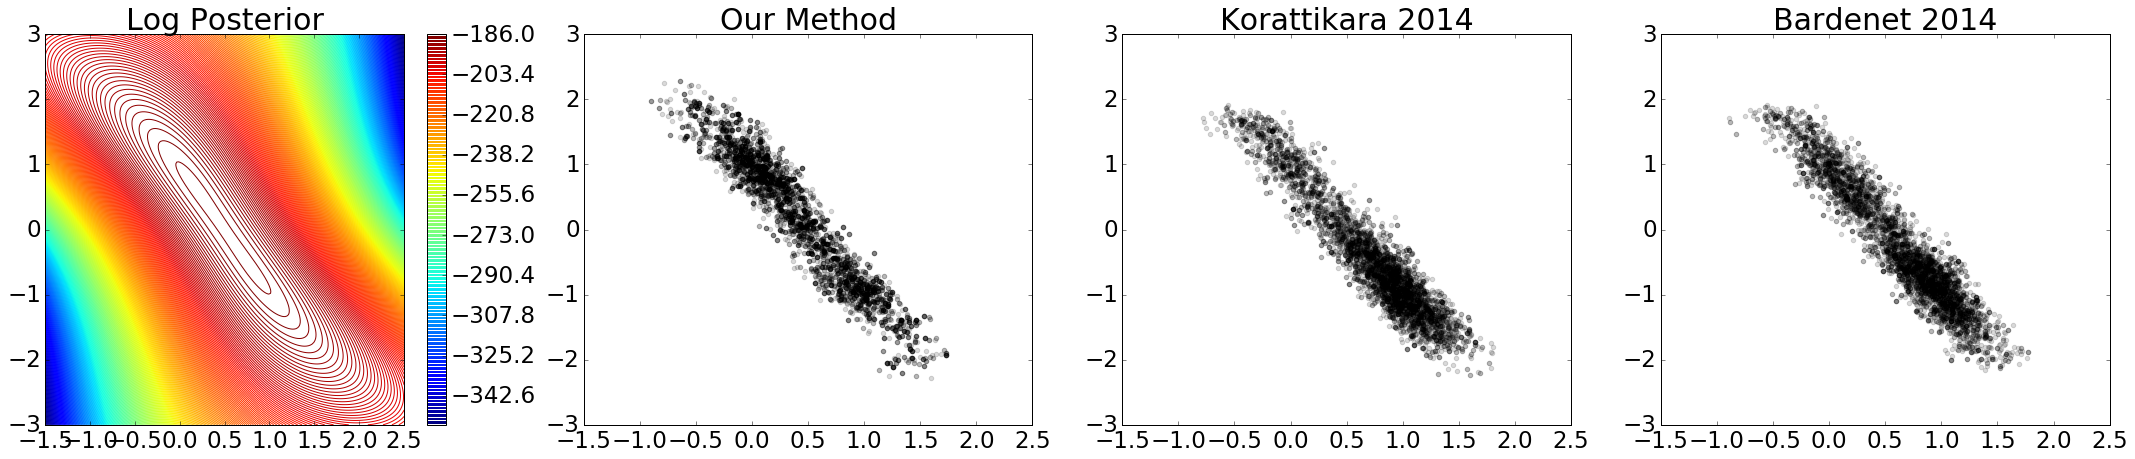
\includegraphics[width=0.9\linewidth]{posterior_of_gaussian.png}
    \caption{
    The log posterior contours and scatter plots of sampled $\theta$ values
    using different methods. 
    }
    \label{fig:gauss_mix_1}
\end{figure*}
\begin{figure*}[t]
    \centering
    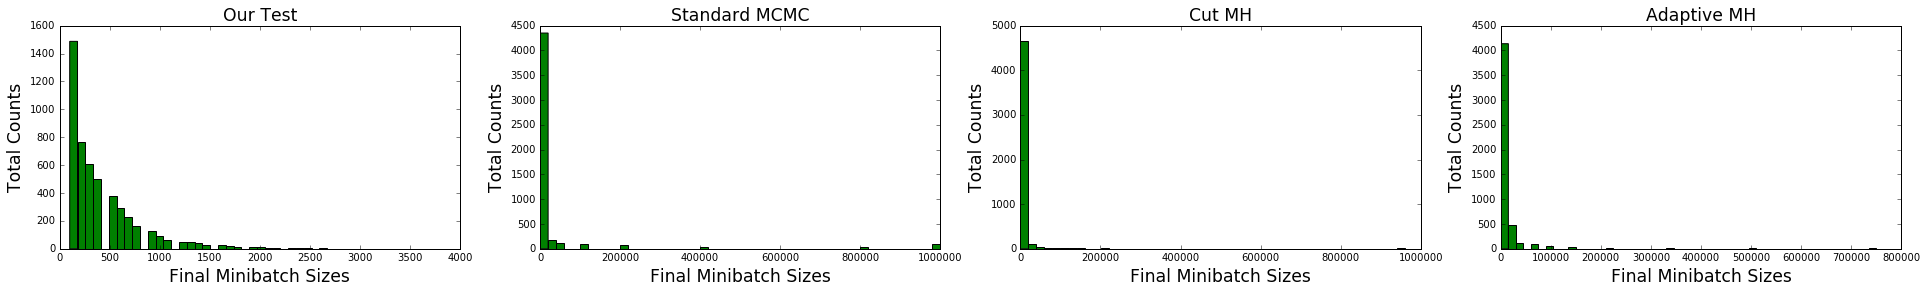
\includegraphics[width=0.9\linewidth]{minibatch_size_gaussian.png}
    \caption{
    Minibatch sizes used in Section~\ref{ssec:gaussians}'s experiment. The axes
    have the same (log-log scale) range.
    }
    \label{fig:gauss_mix_2}
\end{figure*}

This model is adapted from~\cite{langevin_2011} by increasing the number
of samples to 1 million.  The parameters are $\theta = \langle \theta_1,\theta_2 \rangle$, and the
generation process is
\begin{equation}\label{eq:data_generation}
\begin{split}
    \theta &\sim \mathcal{N}(0, {\rm diag}(\sigma_1^2,\sigma_2^2)) \\
    x_i & \sim 0.5 \cdot \mathcal{N}(\theta_1, \sigma_x^2) + 0.5 \cdot \mathcal{N}(\theta_1+\theta_2, \sigma_x^2).
\end{split}
\end{equation}
We set $\sigma_1^2 = 10, \sigma_2^2 = 1$ and $\sigma_x^2=2$.  We fix $\theta =
\langle 0,1 \rangle$. The original paper sampled 100 data points and estimated
the posterior. We are interested in performance on larger problems and so
sampled 1,000,000 points to form the posterior of
$p(\theta)\prod_{i=1}^{1,000,000}p(x_i | \theta)$ with the same prior from
Equation~(\ref{eq:data_generation}). This produces a much sharper posterior with
two very narrow peaks.  Our goal is to reproduce the original posterior, so we
adjust the temperature to $T=10,000$.  Taking logs, we get the target as shown
in the far left of Figure~\ref{fig:gauss_mix_1}.

We ran MCMC with with our test against the test
from~\cite{icml2014c1_bardenet14} and a simplified version
of~\cite{cutting_mh_2014}. Both methods use repeated testing which must be
discounted to bound overall test accuracy. ~\cite{icml2014c1_bardenet14}
conservatively partitions the test error, while~\cite{cutting_mh_2014} used a
complex dynamic programming heuristic to estimate the overall test error. We did
not implement this heuristic and instead set the individual test error equal to
the overall test error. Thus our results for~\cite{cutting_mh_2014} should be
treated as lower bounds. All methods were initialized with minibatch size 100.
For~\cite{cutting_mh_2014} we increment sizes by 100 and set the tolerance
$\epsilon=0.005$ to control overall test error.
For~\cite{icml2014c1_bardenet14}, we increase sizes geometrically with $\gamma =
1.5$ and use parameters $p = 2, \delta = 0.01$.  All methods collect 5000
samples using a random walk proposer with covariance ${\rm diag}(0.15, 0.15)$,
which means the M-H test is responsible for shaping the sample distribution.

Figure~\ref{fig:gauss_mix_1} shows scatter plots of the resulting $\theta$
samples for the three methods, with darker regions indicating a greater density
of points. There are no obvious differences, so we measure the similarity
between each set of samples and the actual posterior. \textbf{Daniel: I think
this was taking up too much space so I put it in Appendix~\ref{app:gaussians}.
Let's state the result (in Table~\ref{tab:poissons}) and prioritize other stuff
here.  TODO}

Figure~\ref{fig:gauss_mix_2} shows that the new method dominates in
terms of speed and efficiency. The histograms of the (final) minibatch sizes
used each iteration show that our method consumes significantly less data; the
distribution is short-tailed and the mean is 210, more than an order of
magnitude better compared to the other two methods (averages are 15562 and
16857). The sizes correspond to the running times of the methods, since
they all consume linear time in data consumed. 


\subsection{Logistic Regression}\label{ssec:logistic}

% Daniel: moving this here so figures don't overflow to next pages. We can tune
% the positioning if needed.
\begin{figure*}[t]
	\centering
	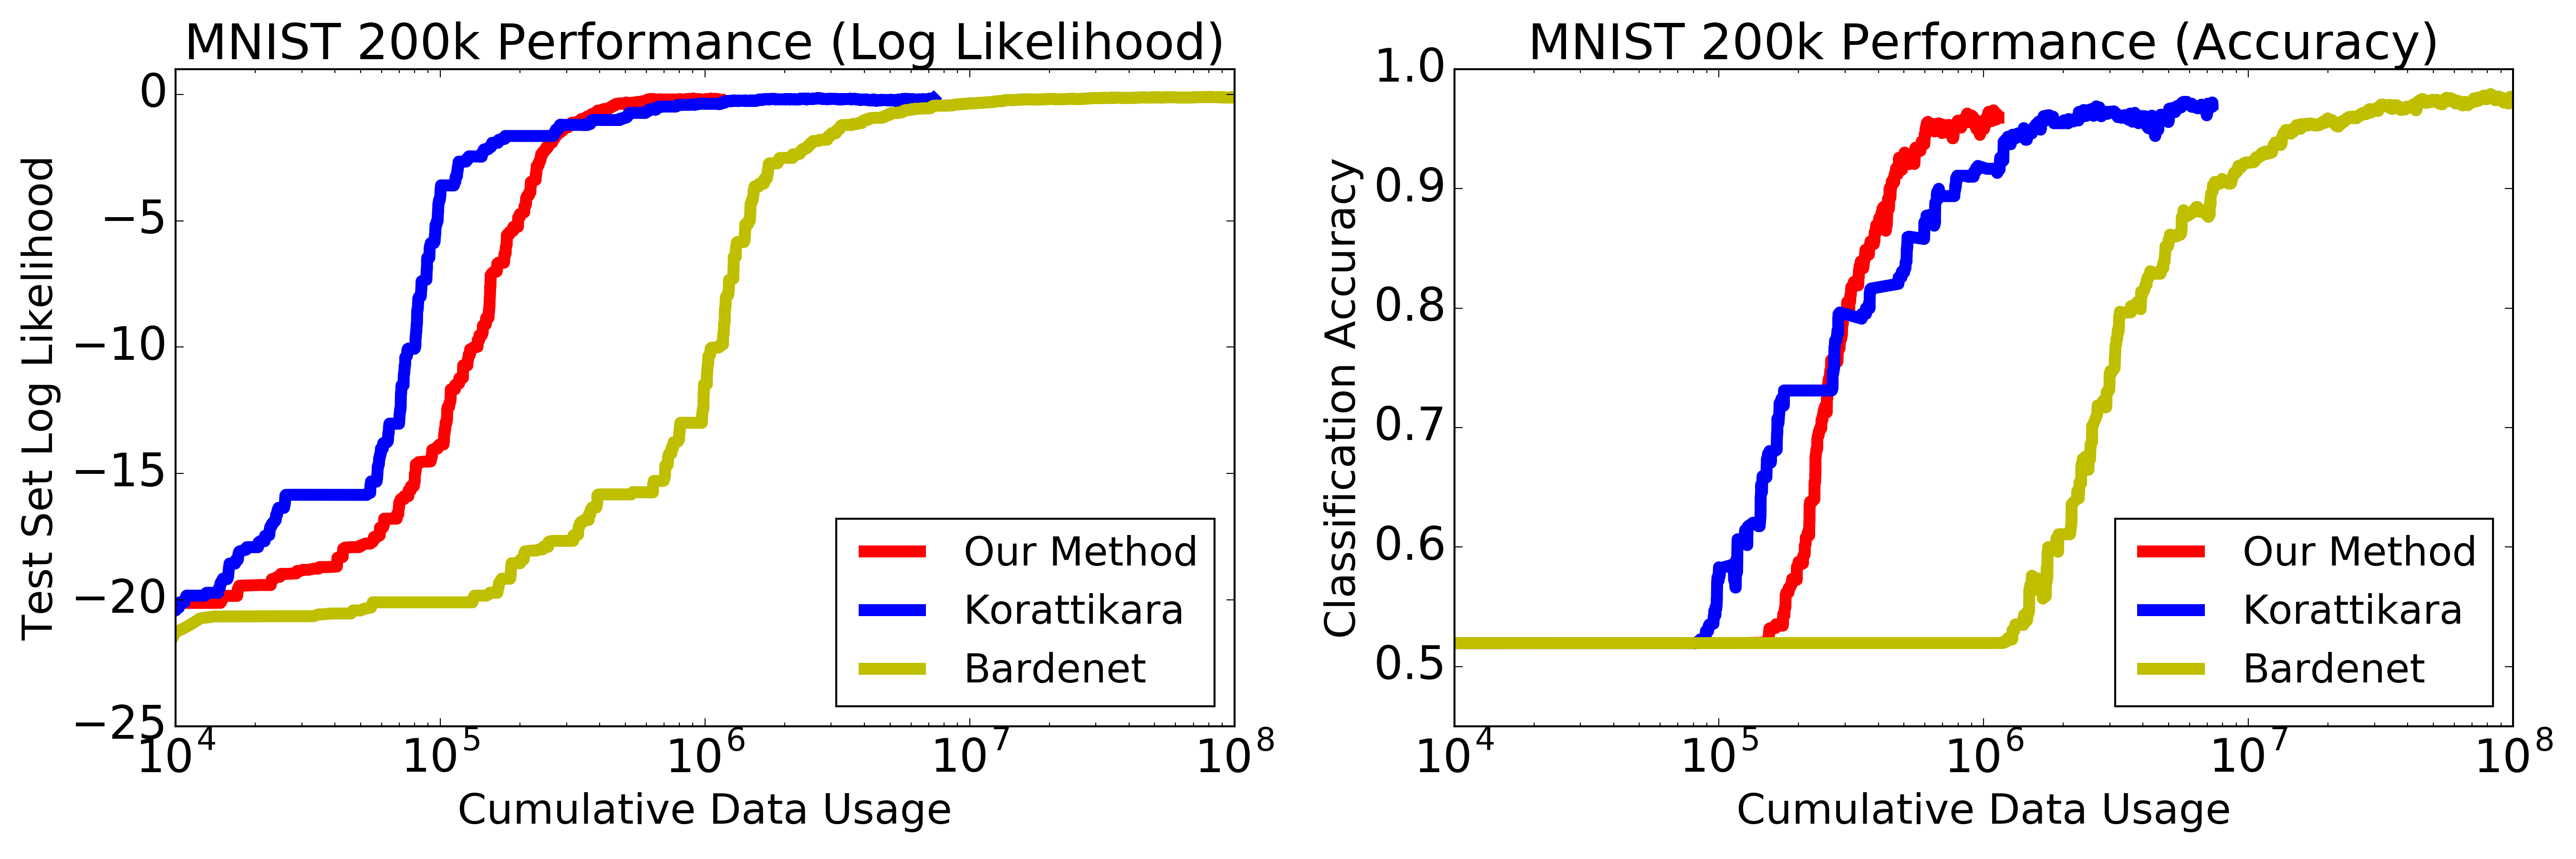
\includegraphics[width=0.9\linewidth]{logistic_regression_ll_acc_results.png}
	\caption{
    Logistic regression performance (accuracy/log likelihood) based on
    cumulative data usage.
    }
	\label{fig:logistic_performance}
\end{figure*}
\begin{figure*}[t]
	\centering
	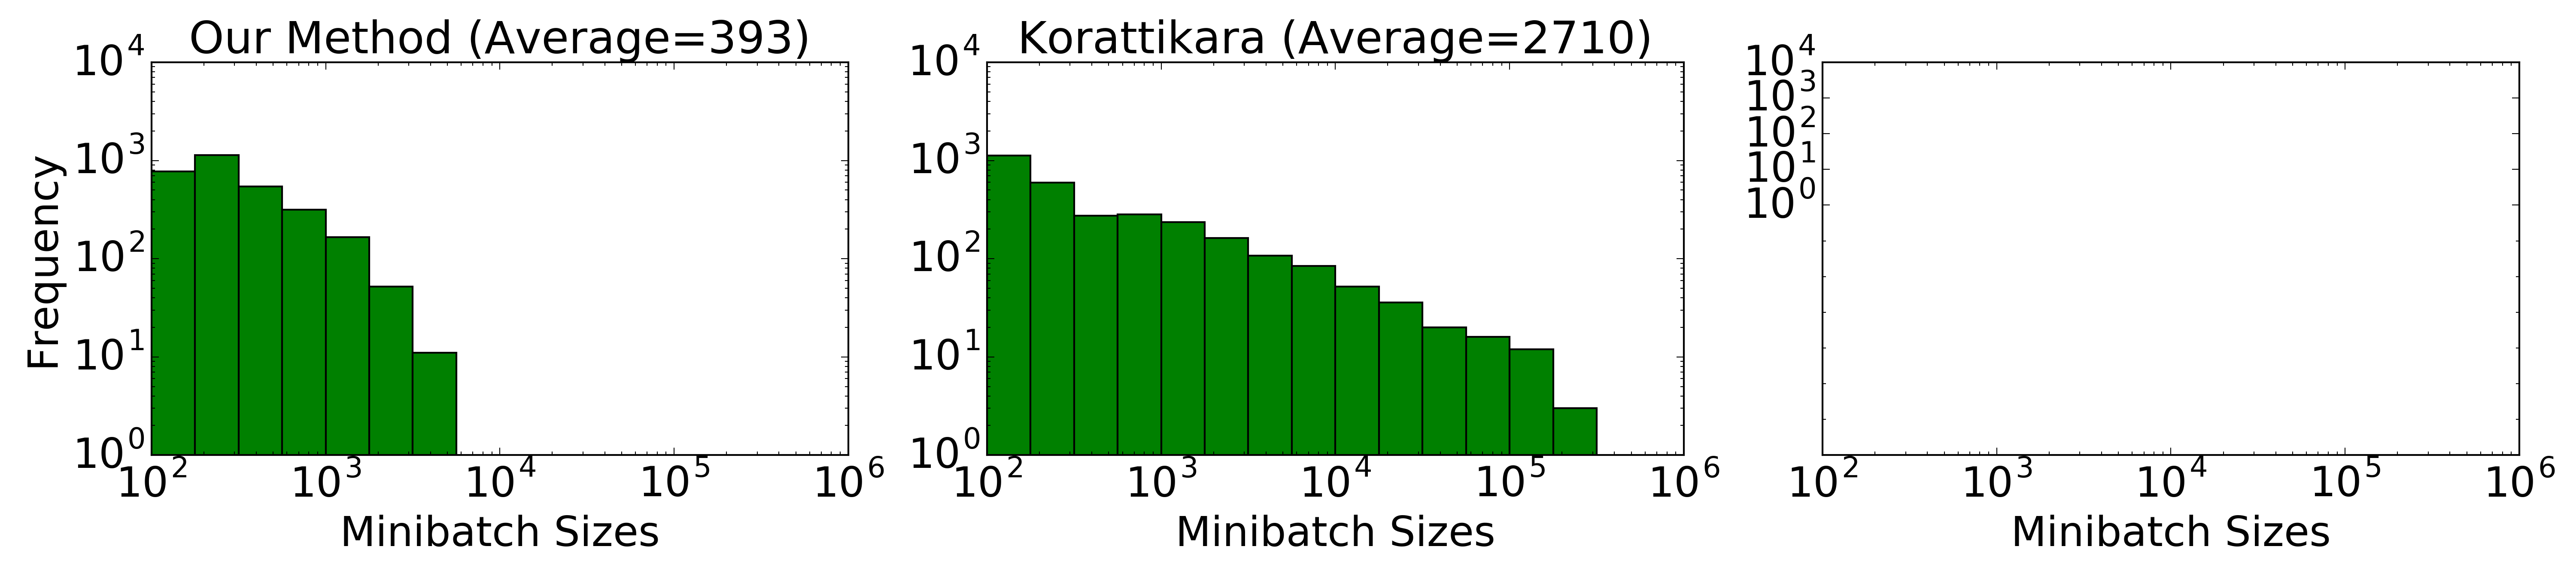
\includegraphics[width=0.9\linewidth]{logistic_regression_histograms_results.png}
	\caption{
    Counts of minibatch sizes in the logistic regression experiment (analogous
    to Figure~\ref{fig:gauss_mix_2}).
    }
	\label{fig:logistic_minibatch}
\end{figure*}

We next test logistic regression for the binary classification of 1s versus 7s
on a subset of the MNIST8M dataset, a larger version of
MNIST~\cite{lecun-mnisthandwrittendigit-2010}. We randomly subsampled 450k
training and 192k testing points.  We impose a uniform prior on $\theta$ and
again use a random walk proposer, this time with covariance matrix $0.05I$. The
temperature is set at $T=1000$. We run the three tests for 3000 samples and
again use 100 as the starting minibatch size. Our undiscounted implementation
of~\cite{cutting_mh_2014} used per-test error of $\epsilon=0.05$.
For~\cite{icml2014c1_bardenet14}, we use their recommended discounting factor
value of $\gamma=2.0$. We tried to use the symbolic bound for
$C_{\theta,\theta'}$ for Logistic regression from~\cite{icml2014c1_bardenet14},
but found it to be too high. Instead we use the empirical $C_{\theta,\theta'}$
from the entire dataset and do not add its computation time when considering
runtime, so again our results represent a lower bound for this method.

Figure~\ref{fig:logistic_performance} shows the test log likelihood and
prediction accuracy as a function of the cumulative training points
processed.\footnote{The curves do not span the same length over the x-axis since
the methods consume different amounts of data.} To generate the curves, for each
of the sampled vectors $\theta_t$, $t\in\{1,\ldots,3000\}$, we use $\theta_t$ as
the parameter for logistic regression.  Our minibatch MH test is more efficient
in terms of accuracy, achieving convergence roughly twice as fast compared
to~\cite{cutting_mh_2014} and about 1.5 orders of magnitude faster
than~\cite{icml2014c1_bardenet14}, though its log likelihood results lag
slightly behind the former algorithm during the very early stages of
exploration.

Figure~\ref{fig:logistic_minibatch} shows histograms of minibatch sizes for the
three methods on a log-log scale. With an initial size of 100, we achieve an
average minibatch size of 393, more than two orders of magnitude smaller
than~\cite{icml2014c1_bardenet14}, and almost an order of magnitude faster than
the undiscounted implementation of~\cite{cutting_mh_2014}.



\subsection{Collaborative Filtering}\label{ssec:collab_filtering}

\textbf{Daniel: TODO we wanted a third experiment, right?}


\section{Conclusions}\label{sec:conclusion}

\textbf{Daniel: need to revise this to take into account reviewer suggestion,
with future work ideas. This will add some 2016 references so that'll be good
(makes it current)}

We have derived an M-H test for minibatch MCMC which approximates full data
tests. We present theoretical results and experimentally show the benefits of
our test on Gaussian mixtures and logistic regression. Directions for future
work include running more experiments with a particular focus on controlling
variances, testing on neural networks, combining our results with Hamiltonian
Monte Carlo methods, providing a recipe for how to use our algorithm (following
the framework of~\cite{sgmcmc_2015}), or integrating parallel
MCMC~\cite{conf/uai/AngelinoKWSA14,conf/icml/AhnSW14} concepts.

\bibliography{paper}
\bibliographystyle{icml2017}

\clearpage
\appendix

% Daniel: I set the Appendix at single column which makes some of the math
% easier to write. Other ICML papers from 2016 did this so it's not a big deal.

\onecolumn
\begin{center}
{\Large Appendix}
\end{center}

This appendix is divided into two main parts. Appendix~\ref{app:proofs} provides
the proofs that we omitted from the main text due to space constraints.
Appendix~\ref{app:experiments} provides further details on the correction
distribution derivation and on our three main experiments to assist
understanding and reproducibility.


\section{Proofs of Lemmas and Corollaries}\label{app:proofs}

\subsection{Proof of Lemma~\ref{lem:worst_case}}\label{app:worst_case_proof}

Choose $(\theta' - \theta) \in \pm\frac{1}{\sqrt{N}}[0.5,1]$ (event 1) and
$(\theta -0.5) \in \pm\frac{1}{\sqrt{N}}[0.5,1]$ filtered for  matching sign
(event 2).  As discussed in Lemma~\ref{lem:worst_case}, both $q(\theta' |
\theta)$ and $p(\theta | x_1,\ldots,x_N)$ have variance $1/N$. If we denote
$\Phi$ as the CDF of the standard normal distribution, then the former event
occurs with probability $p_0 = 2(\Phi(\sqrt{N}\frac{1}{\sqrt{N}}) -
\Phi(\sqrt{N}\frac{0.5}{\sqrt{N}})) = 2(\Phi(1)-\Phi(0.5)) \approx 0.2997$. The
latter event, because we restrict signs, occurs with probability $p_1 =
\Phi(1)-\Phi(0.5) \approx 0.14988$. 

These events together guarantee that $\Lambda^*(\theta,\theta')$ is negative by
inspection of equation (\ref{eq:whyneg}) below.  This implies that we can find a
$u \in (0,1)$ so that $\psi(u,\theta,\theta') = \log u < 0$ equals
$\mE[\Lambda^*(\theta,\theta')]$.  Specifically, choose $u_0$ to satisfy $\log u_0
= \mE[\Lambda^*(\theta,\theta')]$.  Using $\mE[x_i^*] = 0.5$ and
Equation~(\ref{eq:lemma_ll_ratio}), we see that
\begin{equation}
  \log u_0 = N(\theta'-\theta)\frac{1}{b} \cdot \mE\left[\sum_{i=1}^b x_i^*-\theta-\frac{\theta'-\theta}{2}\right]
\end{equation}
\begin{equation}\label{eq:whyneg}
    \log u_0 = -N(\theta'-\theta)\left(\theta-0.5+\frac{\theta'-\theta}{2}\right).
\end{equation}
Next, consider the minibatch acceptance test $\Lambda^*(\theta,\theta')
\not\approx \psi(u,\theta,\theta')$ used in ~\cite{cutting_mh_2014}
and~\cite{icml2014c1_bardenet14} , where $\not\approx$ means ``significantly
different from'' under the distribution over samples. This is
\begin{align}
\Lambda^*(\theta,\theta')  \not\approx \psi(u_0,\theta,\theta') 
&\iff N(\theta'-\theta) \cdot \frac{1}{b}\sum_{i=1}^b x_i^*-\theta-\frac{\theta'-\theta}{2} \not\approx \log u_0\\
&\iff \frac{1}{b}\sum_{i=1}^b x_i^*-\left(\theta+\frac{\theta'-\theta}{2} + \frac{\log u_0}{N(\theta'-\theta)}\right) \not\approx  0 \\
&\iff \frac{1}{b}\sum_{i=1}^b x_i^*-0.5 \not\approx 0. \label{eq:accept_test_zero}
\end{align}
Since the $x_i^*$ have mean 0.5, the resulting test with our chosen $u_0$ will
never correctly succeed and must use all $N$ data points.  Furthermore, if we
sample values of $u$ near enough to $u_0$, the terms in parenthesis will not be
sufficiently different from 0.5 to allow the test to succeed. 
  
The choices above for $\theta$ and $\theta'$ guarantee that
\begin{equation}\label{eq:log_uo_range}
    \log u_0 \in -[0.5,1][0.75,1.5] = [-1.5, -0.375].
\end{equation}
Next, consider the range of $u$ values near $u_0$:
\begin{equation}\label{eq:log_u_range}
    \log u \in \log u_0 + [-0.5,0.375].
\end{equation}
The size of the range in $u$ is at least $\exp([-2,-1.125]) \approx
[0.13534,0.32465]$ and occurs with probability at least $p_2=0.18932$. With $u$
in this range, we rewrite the test as:
\begin{equation}\label{eq:accept_test_rewritten}
    \frac{1}{b}\sum_{i=1}^b x_i^*-0.5 \hspace{0.1in} \not\approx \hspace{0.1in} \frac{\log u/u_0}{N(\theta'-\theta)}
\end{equation}
so that, as in Equation~(\ref{eq:accept_test_zero}), the LHS has expected value
zero.  Given our choice of intervals for the variables, we can compute the range
for the right hand side (RHS) assuming\footnote{If $\theta'-\theta<0$, then the
range would be $\frac{1}{\sqrt{N}}[-0.75,1]$ but this does not matter for
the purposes of our analysis.} that $\theta'-\theta > 0$:
\begin{equation}\label{eq:rhs_range}
\min\{{\rm RHS}\} = \frac{-0.5}{\sqrt{N} \cdot 0.5} = -\frac{1}{\sqrt{N}}
\quad {\rm and} \quad \max\{{\rm RHS}\} = \frac{0.375}{\sqrt{N} \cdot 0.5} = \frac{0.75}{\sqrt{N}}
\end{equation}
Thus, the RHS is in $\frac{1}{\sqrt{N}}[-1,0.75]$.  The standard deviation of
the LHS given the interval constraints is at least $0.5/\sqrt{b}$.
Consequently, the gap between the LHS and RHS in
Equation~(\ref{eq:accept_test_rewritten}) is at most $2\sqrt{b/N}$ standard
deviations, limiting the range in which the test will be able to ``succeed''
without requiring more samples.

The samples $\theta$, $\theta'$ and $u$ are drawn independently and so the
probability of the conjunction of these events is $c = p_0 p_1 p_2 = 0.0085$.


\subsection{Proof of Lemma~\ref{lem:quant_clt}}\label{app:quant_clt}

The following bound is given immediately after Corollary 2 from~\cite{explicit-clt05}:
\begin{equation}
-6.4\mE[|X|^3]-2\mE[|X|] \leq \sup_x|{\rm Pr}(t<x)-\Phi(x)|{\sqrt{n}} \leq
1.36\mE[|X|^3].
\end{equation}
This bound applies to $x\geq 0$. Applying the bound to $-x$ when $x<0$
and combining with $x>0$, we obtain the weaker but unqualified bound
in Equation~(\ref{eq:clt-bounds}).


\subsection{Proof of Lemma~\ref{lem:cdf_bounds}}\label{app:proof_cdf_bounds}

We first observe that
\[
    P'(z) - Q'(z) = \int_{-\infty}^{+\infty}(P(z-x)-Q(z-x))R(x) dx,
\]
and since $\sup_x|P(x)-Q(x)|\leq \epsilon$ it follows that $\forall z$:
\begin{equation}
-\epsilon = \int_{-\infty}^{+\infty} -\epsilon R(x) dx \leq \int_{-\infty}^{+\infty}(P(z-x)-Q(z-x))R(x) dx \leq \int_{-\infty}^{+\infty}\epsilon R(x) dx = \epsilon,
\end{equation}
% Daniel: this is the multi-line version, but we should use the full page.
%\begin{align*}
%-\epsilon &= \int_{-\infty}^{+\infty} -\epsilon R(x) dx \\
%&\leq \int_{-\infty}^{+\infty}(P(z-x)-Q(z-x))R(x) dx \\
%&\leq \int_{-\infty}^{+\infty}\epsilon R(x) dx = \epsilon,
%\end{align*}
as desired.


\subsection{Proof of Corollary~\ref{cor:bounds_preserved}}\label{app:bounds_preserved}

We apply Lemma~\ref{lem:cdf_bounds} twice. First take:
\begin{equation}
    P(y) = {\rm Pr}(\Delta^* < y)
     \quad {\rm and} \quad Q(y) = \Phi\left(\frac{y-\Delta}{s_{\Delta^*}}\right)
\end{equation}
and convolve with the distribution of $X_n$ which has density $\phi(X/\sigma_n)$
where $\sigma_n^2 = 1 - s^2_{\Delta^*}$. This yields the next iteration of $P$
and $Q$:
\begin{equation}
    P'(y) = {\rm Pr}(\Delta^*+X_{\rm nc} < y)
    \quad {\rm and}\quad Q'(y) = \Phi\left({y-\Delta}\right)
\end{equation}
Now we convolve with the distribution of $X_{\rm corr}$:
\begin{equation}
    P''(y) = {\rm Pr}(\Delta^*+X_{\rm nc}+X_{\rm corr} < y)
    \quad {\rm and}\quad Q''(y) = S\left({y-\Delta}\right)
\end{equation}
Both steps preserve the error bound $\epsilon(\theta,\theta',b)$. Finally
$S(y-\Delta)$ is a logistic CDF centered at $\Delta$, and so $S(y-\Delta) =
{\rm Pr}(\Delta + X_{\rm log} < y)$ for a logistic random $X_{\rm log}$. We conclude
that the probability of acceptance for the actual test ${\rm Pr}(\Delta^*+X_{\rm
nc}+X_{\rm corr} > 0)$ differs from the exact test ${\rm Pr}(\Delta+X_{\rm log} > 0)$
by at most $\epsilon$.


\subsection{Improved Error Bounds Based on Skew Estimation}\label{app:better_error_bound}

We show that the CLT error bound can be improved to $O(n^{-1})$ using a more
precise limit distribution under an additional assumption. Let $\mu_i$ denote
the $i^{th}$ moment, and $b_i$ denote the $i^{th}$ absolute moment of $X$. If
Cramer's condition holds:
\begin{equation}\label{eq:cramers_condition}
    \lim_{t \to \infty} \sup |\mE[\exp(i t X)]| < 1,
\end{equation}
then Equation 2.2 in Bentkus et al.'s work on Edgeworth
expansions~\cite{Bentkus97} provides:

\begin{lemma}\label{lem:clt_edgeworth}
Let $X_1,\ldots,X_n$ be a set of zero-mean, independent, identically-distributed
random variables with sample mean $\hat{X}$ and with $t$ defined as in Lemma 3.
If $X$ satisfies Cramer's condition, then
%\begin{equation}\label{eq:clt-bounds_edgeworth}
\[
    \sup_x\left|{\rm Pr}(t<x) - G\left(x, \frac{\mu_3}{b_2^{3/2}}\right)\right| \leq \frac{c(\epsilon,b_2,b_3,b_4,b_{4+\epsilon})}{n}
\]
%\end{equation}
where
\begin{equation}
    G_n(x,y) = \Phi(x) + \frac{y(2x^2+1)}{6\sqrt{n}}\Phi'(x).
\end{equation}
\end{lemma}
Lemma~\ref{lem:clt_edgeworth} shows that the average of the $X_i$ has a more
precise, skewed CDF limit $G_n(x,y)$ where the skew term has weight proportional
to a certain measure of skew derived from the moments:
$\mu_3/b_2^{3/2}$. Note that if the $X_i$ are symmetric, the weight of
the correction term is zero, and the CDF of the average of the $X_i$ converges
to $\Phi(x)$ at a rate of $O(n^{-1})$.

Here the limit $G_n(x,y)$ is a normal CDF plus a correction term that decays as
$n^{-1/2}$.
Importantly, since $\phi^{''}(x) = x^2\phi(x) - \phi(x)$ where
$\phi(x)=\Phi'(x)$, the correction term can be rewritten giving:
\begin{equation}\label{eq:GNderivatives}
    G_n(x,y) = \Phi(x) + \frac{y}{6\sqrt{n}}(2\phi^{''}(x)+3\phi(x))
\end{equation}
From which we see that $G_n(x,y)$ is a linear combination of $\Phi(x)$,
$\phi(x)$ and $\phi^{''}(x)$. In Algorithm 1, we
correct for the difference in $\sigma$ between $\Delta^*$ and the variance
needed by $X_{\rm corr}$ using $X_{\rm nc}$. This same method works when we
wish to estimate the error in $\Delta^*$ vs $G_n(x,y)$. Since all of the
component functions of $G_n(x,y)$ are derivatives of a (unit variance)
$\Phi(x)$, adding a normal variable with variance $\sigma'$ increases the
variance of all three functions to $1+\sigma'$. Thus we add $X_{\rm nc}$ as
per Algorithm 1 preserving the limit in Equation~(\ref{eq:GNderivatives}).

The deconvolution approach can be used to construct a correction variable
$X_{\rm corr}$ between $G_n(x,y)$ and $S(x)$ the standard logistic function. An
additional complexity is that $G_n(x,y)$ has additional parameters $y$ and $n$.
Since these act as a single multiplier $\frac{y}{6\sqrt{n}}$ in
Equation~(\ref{eq:GNderivatives}), its enough to consider a function $g(x,y')$
parametrized by $y'= \frac{y}{6\sqrt{n}}$. This function can be computed and
saved offline. As we have shown earlier, errors in the ``limit'' function
propagate directly through as errors in the acceptance test.  To achieve a test
error of $10^{-6}$ (close to single floating point precision), we need a $y'$
spacing of $10^{-6}$. It should not be necessary to tabulate values all the way to
$y'=1$, since $y'$ is scaled inversely by the square root of minibatch size.
Assuming a max $y'$ of 0.1 requires us to tabulate about 100,000.  Since our $x$
resolution is 10,000, this leads to a table with about 1 billion values, which
can comfortably be stored in memory.  However, if $g(x,y)$ is moderately smooth
in $y$, it should be possible to achieve similar accuracy with a much smaller
table. We leave further analysis and experiments with $g(x,y)$ as future work.





\section{Additional Experiment Details}\label{app:experiments}
% Daniel: all three experiments should be described in more detail here. And
% also the deconvolution step to get the correction distribution.

\subsection{Obtaining the Correction Distribution (Section~\ref{sec:correction})}\label{app:correction}

% Daniel: moved to appendix so we can expand it. Originally we had only two
% lines, and it looked pretty awkward. So let's add more. Note: this also
% depends on whether we use [-10,10] for the X_c range, or [-20,20], etc...
\begin{table}[t]
\caption{Errors ($L_\infty$) in $X_{\rm norm}+X_{\rm corr}$ versus $X_{\rm
log}$, with $N=4000$ (top row) and $N=2000$ (bottom row).}
\label{tab:xcorr}
\vskip 0.15in
\begin{center}
\begin{small}
\begin{sc}
%% ----------------------- START OF TABLE
\begin{tabular}{l l}
\hline
\abovespace\belowspace
$N=4000$ & $\sigma=1.1$ \\
\hline
\abovespace\belowspace
$\lambda$ & $L_{\infty}$ error \\
\hline
\abovespace
100    & \textbf{4.3e-3}  \\
10     & 6.0e-3  \\
1      & 1.0e-2  \\
0.1    & 1.2e-2  \\
\belowspace
0.01   & 3.5e-2  \\
\hline
\end{tabular}
\quad %% ----------------------- START OF TABLE
\begin{tabular}{l l}
\hline
\abovespace\belowspace
$N=4000$ & $\sigma=1.0$ \\
\hline
\abovespace\belowspace
$\lambda$ & $L_{\infty}$ error \\
\hline
\abovespace
100    & 1.9e-3  \\
10     & \textbf{8.9e-4}  \\
1      & 1.6e-3  \\
0.1    & 2.8e-3  \\
\belowspace
0.01   & 5.2e-3  \\
\hline
\end{tabular}
\quad %% ----------------------- START OF TABLE
\begin{tabular}{l l}
\hline
\abovespace\belowspace
$N=4000$ & $\sigma=0.9$ \\
\hline
\abovespace\belowspace
$\lambda$ & $L_{\infty}$ error \\
\hline
\abovespace
100    & 1.2e-3  \\
10     & 2.6e-4  \\
1      & \textbf{1.0e-4}  \\
0.1    & 2.0e-4  \\
\belowspace
0.01   & 3.9e-4  \\
\hline
\end{tabular}
\quad %% ----------------------- START OF TABLE
\begin{tabular}{l l}
\hline
\abovespace\belowspace
$N=4000$ & $\sigma=0.8$ \\
\hline
\abovespace\belowspace
$\lambda$ & $L_{\infty}$ error \\
\hline
\abovespace
100    & 8.3e-4  \\
10     & 1.3e-4  \\
1      & 2.5e-5  \\
0.1    & \textbf{6.7e-6}  \\
\belowspace
0.01   & 7.4e-6  \\
\hline
\end{tabular}
%% ---- NEW ROW ----
\vskip 0.2in %% OH this works!
\begin{tabular}{l l}
\hline
\abovespace\belowspace
$N=2000$ & $\sigma=1.1$ \\
\hline
\abovespace\belowspace
$\lambda$ & $L_{\infty}$ error \\
\hline
\abovespace
100    & 6.8e-3  \\
10     & \textbf{4.6e-3}  \\
1      & 7.5e-3  \\
0.1    & 1.3e-2  \\
\belowspace
0.01   & 2.4e-2  \\
\hline
\end{tabular}
\quad %% ----------------------- START OF TABLE
\begin{tabular}{l l}
\hline
\abovespace\belowspace
$N=2000$ & $\sigma=1.0$ \\
\hline
\abovespace\belowspace
$\lambda$ & $L_{\infty}$ error \\
\hline
\abovespace
100    & 4.4e-3  \\
10     & 1.3e-3  \\
1      & \textbf{1.1e-3}  \\
0.1    & 2.0e-3  \\
\belowspace
0.01   & 3.6e-3  \\
\hline
\end{tabular}
\quad %% ----------------------- START OF TABLE
\begin{tabular}{l l}
\hline
\abovespace\belowspace
$N=2000$ & $\sigma=0.9$ \\
\hline
\abovespace\belowspace
$\lambda$ & $L_{\infty}$ error \\
\hline
\abovespace
100    & 3.3e-3  \\
10     & 6.4e-4  \\
1      & 1.6e-4  \\
0.1    & \textbf{1.3e-4}  \\
\belowspace
0.01   & 2.7e-4  \\
\hline
\end{tabular}
\quad %% ----------------------- START OF TABLE
\begin{tabular}{l l}
\hline
\abovespace\belowspace
$N=2000$ & $\sigma=0.8$ \\
\hline
\abovespace\belowspace
$\lambda$ & $L_{\infty}$ error \\
\hline
\abovespace
100    & 2.6e-3  \\
10     & 4.0e-4  \\
1      & 6.7e-5  \\
0.1    & 1.4e-5  \\
\belowspace
0.01   & \textbf{5.0e-6}  \\
\hline
\end{tabular}
\end{sc}
\end{small}
\end{center}
\vskip -0.1in
\end{table}


\textbf{Daniel: TODO, figure out what values to test, put optimal values in bold
face here, etc., note that these are with the range $[-20,20]$ except for the
best value in $[-10,10]$; maybe we should decrease the range?}

\subsection{Gaussian Mixture Model Experiment (Section~\ref{ssec:gaussians})}\label{app:gaussians}

\begin{table}[t]
\caption{Gaussian Mixture Model Statistics}
\label{tab:poissons}
\vskip 0.15in
\begin{center}
\begin{small}
\begin{sc}
\begin{tabular}{l l l l}
\hline
\abovespace\belowspace
Metric & Ours & Korat.'14 & Barde.'14 \\
\hline
\abovespace
Equation~\ref{eq:log_prob_poissons} & -1430.0 & -1578.9 & -1232.7 \\
\belowspace
Chi-Squared & 3313.9 & 3647.7 & 2444.1 \\
\hline
\end{tabular}
\end{sc}
\end{small}
\end{center}
\vskip -0.1in
\end{table}

We discretize the posterior coordinates into bins with respect to the two
components of $\theta$.  The probability $P_i$ of a sample falling into bin $i$
is the integral of the true posterior over the bin's area.  A single sample
should therefore be multinomial with distribution $P$, and a set of $n$ (ideally
independent) samples is ${\rm Multinomial}(P,n)$. This distribution is simple
and we can use it to measure the quality of the samples rather than use general
purpose tests like KL-divergence or likelihood-ratio, which are problematic
with zero counts.

For large $n$, the per-bin distributions are approximated by Poissons with
parameter $\lambda_i=P_i n$. Given samples $\{\theta_1,\ldots,\theta_T\}$, let
$c_j$ denote the number of individual samples $\theta_i$ that fall in bin $j$
out of $N_{\rm bins}$ total. We have
\begin{equation}\label{eq:log_prob_poissons}
\begin{split}
    \log p(c_1, \ldots, c_{N_{\rm bins}} | P_1, \ldots, P_{N_{\rm bins}}) & =  \\
    \sum_{j=1}^{N_{\rm bins}} c_j \log (n P_j) - n P_j - \log(\Gamma(c_j+1)). & \\
\end{split}
\end{equation}
Table~\ref{tab:poissons} shows the likelihoods. To facilitate
interpretation we perform significance tests using Chi-Squared
distribution (also in Table~\ref{tab:poissons}). Scores lie
between~\cite{cutting_mh_2014} and~\cite{icml2014c1_bardenet14}, but
the variance of these values is high and ordering changes depending on
the range of samples generated.

\textbf{Daniel: TODO improve this}

\subsection{Logistic Regression Experiment (Section~\ref{ssec:logistic})}\label{app:logistic}

\textbf{Daniel: TODO}

\subsection{Collaborative Filtering Experiment (Section~\ref{ssec:collab_filtering})}\label{app:collab_filtering}

\textbf{Daniel: TODO}




\end{document} 

% Daniel: some notes to keep in mind to standardize to ICML format.

%% \begin{figure}[ht]
%% \vskip 0.2in
%% \begin{center}
%% \centerline{\includegraphics[width=\columnwidth]{icml_numpapers}}
%% \caption{Historical locations and number of accepted papers for International
%%   Machine Learning Conferences (ICML 1993 -- ICML 2008) and
%%   International Workshops on Machine Learning (ML 1988 -- ML
%%   1992). At the time this figure was produced, the number of
%%   accepted papers for ICML 2008 was unknown and instead estimated.}
%% \label{icml-historical}
%% \end{center}
%% \vskip -0.2in
%% \end{figure} 
%% 
%% \subsection{Figures}
%%  
%% You may want to include figures in the paper to help readers visualize
%% your approach and your results. Such artwork should be centered,
%% legible, and separated from the text. Lines should be dark and at
%% least 0.5~points thick for purposes of reproduction, and text should
%% not appear on a gray background.
%% 
%% Label all distinct components of each figure. If the figure takes the
%% form of a graph, then give a name for each axis and include a legend
%% that briefly describes each curve. Do not include a title inside the
%% figure; instead, the caption should serve this function.
%% 
%% Number figures sequentially, placing the figure number and caption
%% {\it after\/} the graphics, with at least 0.1~inches of space before
%% the caption and 0.1~inches after it, as in
%% Figure~\ref{icml-historical}.  The figure caption should be set in
%% 9~point type and centered unless it runs two or more lines, in which
%% case it should be flush left.  You may float figures to the top or
%% bottom of a column, and you may set wide figures across both columns
%% (use the environment {\tt figure*} in \LaTeX), but always place
%% two-column figures at the top or bottom of the page.
%% 
%% \subsection{Tables} 
%%  
%% You may also want to include tables that summarize material. Like 
%% figures, these should be centered, legible, and numbered consecutively. 
%% However, place the title {\it above\/} the table with at least 
%% 0.1~inches of space before the title and the same after it, as in 
%% Table~\ref{sample-table}. The table title should be set in 9~point 
%% type and centered unless it runs two or more lines, in which case it
%% should be flush left.
%% 
%% % Note use of \abovespace and \belowspace to get reasonable spacing 
%% % above and below tabular lines. 
%% 
%% \begin{table}[t]
%% \caption{Classification accuracies for naive Bayes and flexible 
%% Bayes on various data sets.}
%% \label{sample-table}
%% \vskip 0.15in
%% \begin{center}
%% \begin{small}
%% \begin{sc}
%% \begin{tabular}{lcccr}
%% \hline
%% \abovespace\belowspace
%% Data set & Naive & Flexible & Better? \\
%% \hline
%% \abovespace
%% Breast    & 95.9$\pm$ 0.2& 96.7$\pm$ 0.2& $\surd$ \\
%% Cleveland & 83.3$\pm$ 0.6& 80.0$\pm$ 0.6& $\times$\\
%% Glass2    & 61.9$\pm$ 1.4& 83.8$\pm$ 0.7& $\surd$ \\
%% Credit    & 74.8$\pm$ 0.5& 78.3$\pm$ 0.6&         \\
%% Horse     & 73.3$\pm$ 0.9& 69.7$\pm$ 1.0& $\times$\\
%% Meta      & 67.1$\pm$ 0.6& 76.5$\pm$ 0.5& $\surd$ \\
%% Pima      & 75.1$\pm$ 0.6& 73.9$\pm$ 0.5&         \\
%% \belowspace
%% Vehicle   & 44.9$\pm$ 0.6& 61.5$\pm$ 0.4& $\surd$ \\
%% \hline
%% \end{tabular}
%% \end{sc}
%% \end{small}
%% \end{center}
%% \vskip -0.1in
%% \end{table}
%%
%% % Acknowledgements should only appear in the accepted version. 
%% \section*{Acknowledgements} 
%% \textbf{Do not} include acknowledgements in the initial version of
%% the paper submitted for blind review.
